\chapter{Fahrradtunnel}
Gerade im dicht verbauten Grazer Stadtgebiet rund um das Zentrum ist oft nicht ausreichend Platz für große Fahrradinfrastruktur vorhanden. Oft ist es möglich, auf Kosten anderer Verkehrsteilnehmer die Radinfrastruktur auszubauen, doch das stößt an seine Grenzen.

Eine der Lösungen dafür sind unterirdische Tunnel ausschließlich für den Fahrrad-Verkehr.

Die Vorteile liegen auf der Hand:
\begin{itemize}
    \item Schnelle Direktverbindung
    \item Fahrräder werden nicht durch andere Verkehrsteilnehmer ausgebremst
    \item Andere Verkehrsteilnehmer werden nicht durch Fahrräder ausgebremst
    \item Tunnel sind eine wetterfeste Option
\end{itemize}

Die Nachteile sind jedoch auf der anderen Seite ebenfalls offensichtlich:
\begin{itemize}
    \item Sehr teuer
    \item Unflexibel -- Zu- und Ausfahrt sind nur an bestimmten Stellen möglich
    \item Jede Zufahrt braucht eine flache, raumintensive Rampe
\end{itemize}

Tunnel sind deswegen nur an ausgewählten Stellen möglich und sinnvoll, wo einerseits auf der Oberfläche wirklich nicht ausreichend Platz ist, und auf der anderen Seite ein hohes Potential gegeben ist.

Überlegenswert ist auch, ob man die Tunnel -- je nach Ort, noch breiter ausbaut, um sie auch für Fußgänger als attraktive Alternative zu öffnen.

\section{Portale/Zufahrten}
Eine Zufahrt zu einem Fahrradtunnel muss eine Einfahrt sein, die sowohl bergauf als auch bergab bewältigbar ist. Wie steil diese Einfahrt sein darf, hängt natürlich auch davon ab, wie tief unter der Erde der Tunnel sein muss -- und das hängt von (unter anderem) folgenden Faktoren ab:
\begin{itemize}
    \item Umliegende Keller oder Tiefgaragen
    \item Kanalsystem
    \item Weitere vergrabene Leitungen (Strom, Internet, etc.)
    \item Wasserläufe
    \item Bodenbeschaffenheit
\end{itemize}

Ein Tunnelportal muss deswegen immer so lang wie möglich sein, um die Steigung so gering wie möglich zu halten. Je nach Platzangebot ist das unterschiedlich schwer zu erreichen.

\paragraph{Was weichen muss}
Ein Tunnelportal nimmt zwangsläufig Platz weg, der sonst anders verwendbar gewesen wäre (und höchstwahrscheinlich anderweitig in Verwendung ist). Bevorzugt sollen dafür Parkflächen weichen, da deren Bedarf durch eine bessere Erreichbarkeit mit dem Fahrrad sowieso sinken sollte. Ist das nicht möglich, soll jeder Platz verwendet werden, der verwendet werden kann, auch Parkanlagen. Das Portal soll dabei möglichst lange überdacht geführt werden und dann begrünt sein. Auch Straßen, wenn eine andere Lösung für den MIV vorliegt, können dafür verwendet werden.

\section{Route 1: Fahrradtunnel Universitäten}
Folgende Route schlagen wir als Hauptverbindung im Grazer Osten in Tunnelform vor:

\begin{itemize}
    \item Inffeldgasse
    \item Neue Technik
    \item Alte Technik
    \item Lichtenfelsgasse
    \item KFU Hauptgebäude (Kreuzung mit Route 2)
    \item Kreuzschwestern-Park
    \item Wirtschaftskammer/Campus02
\end{itemize}

\begin{figure}
    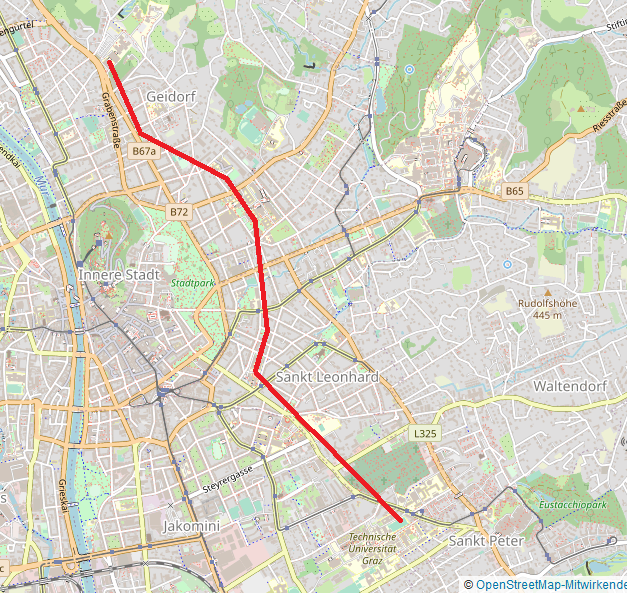
\includegraphics[width=0.8\textwidth]{main/bike/tunnel/uni/linie1}
    \centering
    \caption[Verlauf Linie 1]{Verlauf der Linie 1 zwischen den Zufahrten}
\end{figure}

Zwischen den einzelnen Universitäten findet oft besonders reger Radverkehr statt, und auf dieser Achse ist aufgrund der Bauweise der Stadt oft besonders wenig Platz für Radinfrastruktur.

Dieser Tunnel stellt eine Achse Nord-Süd dar und ist mit einer Kreuzung sowohl mit dem Stadtzentrum als auch dem Landeskrankenhaus verbunden.

\subsection{Zufahrt Inffeldgasse}

\subsection{Mögliche Verlängerung nach Süden}
Von der Zufahrt Inffeldgasse aus ist eine Verlängerung nach Süden denkbar mit folgenden weiteren Zufahrten:
\begin{itemize}
    \item ORF-Park
    \item Wohnpark St. Peter
    \item Messendorf
    \item Raaba
\end{itemize}

\subsection{Mögliche Verlängerung nach Norden}
Von der Zufahrt Wirschaftskammer aus ist eine weitere Verlängerung in Richtung Norden denkbar mit folgenden weiteren Zufahrten:
\begin{itemize}
    \item Ortweinschule
\end{itemize}

Von dort aus ist das Radwegenetz auch oberirdisch gut möglich und teilweise bereits ausgebaut.
\section{Route 2: Fahrradtunnel Innenstadt -- LKH}
Eine weitere mögliche Route mit potentiell hohem Fahrradverkehrsaufkommen und wenig Platz auf der Oberfläche ist eine Verbindung vom LKH in die Innenstadt, von wo eine Direktverbindung zum Murradweg möglich sein kann und soll.

Folgende Zufahrten sind hier geplant:
\begin{itemize}
    \item LKH
    \item Universität Hauptgebäude (Kreuzung mit Route 1)
    \item Stadtpark Murpromenade
\end{itemize}


